\documentclass[sigconf,balance=false]{acmart}
\usepackage{booktabs}
\usepackage{subcaption}
\usepackage{xcolor}
\newcommand{\term}[1]{\emph{#1}}
\newcommand{\refsitem}[1]{\par\noindent\hangindent=1.8em\hangafter=1 #1}
\newenvironment{findingbox}{\par\vskip 3pt\noindent\begin{minipage}{\linewidth}}{\end{minipage}\par\vskip 3pt}
\setlength{\emergencystretch}{1.5em}

\settopmatter{printacmref=false}
\renewcommand\footnotetextcopyrightpermission[1]{}
\pagestyle{plain}
\raggedbottom
\acmConference[Preprint]{Preprint}{October 2026}{}

\begin{document}

\title[What Is Actually Compressible?]{What Is Actually Compressible? An Empirical Study of Context Compression Opportunities in Coding-Agent Trajectories}

\author{Qing Sun}
\affiliation{\institution{Independent Researcher}}

\keywords{coding agents, context compression, empirical measurement, agent trajectories, LLM agents}

\ccsdesc[500]{Software and its engineering~Software verification and validation}
\ccsdesc[300]{Computing methodologies~Artificial intelligence}

\begin{abstract}
Coding agents accumulate repeated and structurally redundant context: tool outputs, file contents, diagnostics, and command results re-enter the conversation as the agent iterates. Context compression is an attractive lever on token cost, yet existing work largely asks \emph{how} to compress; the natural compression-opportunity structure of real coding-agent trajectories remains insufficiently characterized. We present a large-scale empirical characterization built on 35{,}000 trajectories from two independent public corpora---Thoughtworks agentic-coding-trajectories (15{,}000) and NVIDIA Open-SWE-Traces v1.0 Minimax strata (20{,}000)---and a further cross-model analysis on 35{,}334 Qwen3.5-122B trajectories spanning two agent scaffolds (OpenHands, SWE-agent). We derive a 15-shape compression-opportunity taxonomy with deterministic, frozen detectors and apply it across corpora through corpus-specific schema adapters: 8 of 13 measurable shapes satisfy our pre-specified descriptive replication criterion (REPLICATED or PARTIAL)---all six core shapes replicate with full-precision incidence ratios 0.79--1.28---while the five sparse shapes (E6, E7, E10, E11, E15) are corpus-composition-sensitive (DATASET\_SPECIFIC); large diagnostics reach 72.9\% (TW) / 79.5\% (OSW) incidence and late-trajectory large outputs 58.7\% / 46.6\%. Core repeated-delivery shapes are model-stable within both scaffolds (ratios 0.68--1.013), while one shape's incidence is strongly modulated by scaffold (mean scaffold-associated variation 28.2\,pp vs.\ model-associated 12.7\,pp; interaction 16.5\,pp). Mapping shapes to capabilities shows that shipped mechanisms in the evaluated compression system cover only SOC 2.07\% of opportunity-bearing sessions and event-payload COC 0.018\%, whereas a reversible research candidate reaches SOC 100\% and event-payload COC 95.96\% respectively---a 99.98\% relative allocation gap. These findings indicate that context compression should account for empirical workload structure and scaffold behavior rather than be treated as a generic token-reduction problem. A same-caliber recalculation of the four repetition shapes under a unified path-aware normalization shifted discovery-side incidence by at most 3.74\,pp and left all replication bands unchanged on the pre-amendment frame; the discovery census reported here reflects the recovered full three-source parse.
\end{abstract}

\maketitle

\section{Introduction}

Coding agents solve software-engineering tasks by iterating through long tool-use loops: they read source files, run tests, inspect failures, edit code, rerun tests, reread files, and inspect new outputs. Every step appends tool results to the conversation. The consequence is not only a context-window capacity problem: \textbf{information the model has already observed keeps re-entering subsequent context in near-original form}, and much of it is repeated, structurally redundant, or delivered late in the trajectory where its downstream consumption is limited.

Context compression is the natural lever on this cost. Prior work has identified broad forms of waste in coding-agent trajectories and proposed mechanisms to reduce them, reporting substantial token and cost savings~\cite{agentdiet2026}. Yet what is still missing is a systematic, reproducible characterization of the fine-grained opportunity structure: which forms occur naturally, how prevalent they are, whether they replicate across trajectory corpora, and how their incidence varies across models and agent scaffolds. Without this characterization, mechanism design targets whatever is easy to fold rather than what the workload actually contains; a 60\%-incidence opportunity and a 0.01\% curiosity look identical on a benchmark; and the distance between offline savings and online task-level effects remains unexplained.

This paper answers that question empirically. We derive a 15-shape compression-opportunity taxonomy with deterministic detectors, freeze it before any external use, and apply it to 35{,}000 trajectories from two independent public corpora, across two agent scaffolds and two backbone models, through corpus-specific schema adapters; a same-caliber recalculation (pre-amendment frame) bounds the normalization-caliber effect on the repetition shapes. We then map the opportunity surface onto the capabilities of a real compression system to quantify what current deployments would actually cover. Our study answers five research questions:

\begin{itemize}
\item \textbf{RQ1 (Prevalence).} What compression opportunities naturally occur in coding-agent trajectories, and how prevalent are they?
\item \textbf{RQ2 (Cross-corpus reproducibility).} Do these opportunity structures replicate across independent coding-agent trajectory corpora?
\item \textbf{RQ3 (Cross-model stability).} Do the major opportunity structures persist across backbone models?
\item \textbf{RQ4 (Scaffold modulation).} How does agent scaffold design affect opportunity incidence?
\item \textbf{RQ5 (Capability coverage).} How much of the naturally occurring opportunity space is covered by the deployed and candidate capabilities of the evaluated compression system?
\end{itemize}

A secondary finding (F1) quantifies why offline compressibility does not translate into online task-level token savings in our regime.

\textbf{Contributions.}
(1)~A fine-grained, detector-backed compression-opportunity taxonomy (15 shapes) with deterministic, frozen detectors.
(2)~External validation on a second corpus: 8 of 13 measurable shapes satisfy our pre-specified descriptive replication criterion (REPLICATED or PARTIAL)---including all six core shapes (full-precision ratios 0.79--1.28)---while the five sparse shapes (E6, E7, E10, E11, E15) are DATASET\_SPECIFIC (corpus-composition-sensitive).
(3)~A controlled scaffold\,$\times$\,model analysis showing scaffold-associated variation dominates model-associated variation for the highest-incidence late-trajectory shape.
(4)~A dual-ledger opportunity-to-capability gap quantification separating production coverage from research-candidate coverage.

\section{Background and Motivation}

\subsection{Agent Context Growth}

A coding-agent trajectory alternates model actions with environment observations. As the loop iterates, observations accumulate: file listings and file contents from exploration, test and build output from verification, diagnostics from failures, and---repeatedly---the \emph{same} files and the \emph{same} commands as the agent edits and re-verifies. Context growth is therefore not uniform; it is shaped by the \emph{structure} of what the agent chooses to observe.
\begin{figure}[t]
\centering
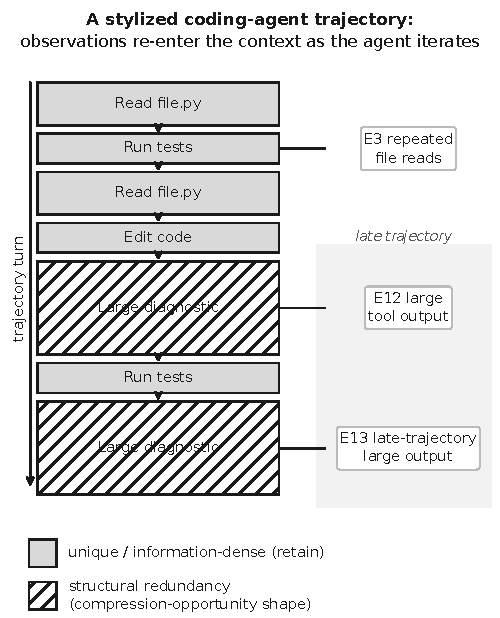
\includegraphics[width=\linewidth]{figures/fig1_trajectory.pdf}
\caption{A coding-agent trajectory annotated with compression opportunities. Repeated file reads (E3), large tool outputs (E12), and late-trajectory large outputs (E13) naturally accumulate as the agent iterates. Not all large observations are redundant; the taxonomy distinguishes structural redundancy from information-dense unique content.}
\Description{Stylized timeline of a coding-agent trajectory. Bars represent tool observations per turn; hatched repeated blocks are annotated E3 repeated file reads, a tall mid-trajectory block is annotated E12 large tool output, and tall late-trajectory blocks are annotated E13 late-trajectory large outputs. A legend distinguishes unique information-dense observations from structural redundancy.}
\label{fig:trajectory}
\end{figure}

\subsection{Compression Opportunity (Definition)}

A \term{compression opportunity} is a trajectory position where an observation contains content that can be represented more compactly \emph{by reference to information already delivered, structural relations among repeated elements, or a more compact equivalent form}. This definition is deliberately conservative: detecting an opportunity does not imply the content is safe to delete, that semantic equivalence holds, or that the model would not need the information again. Opportunity is a \emph{measurement} concept; safety and benefit are separate properties that must be established per mechanism (\S\ref{sec:f1}).

\subsection{Why Opportunity First}

Mechanism-first evaluation answers ``how much does this compressor save on this benchmark?'' Opportunity-first measurement answers ``what does this workload actually contain, how often, with what downstream risk, and what part of it does existing machinery address?'' Only the second question can tell us whether a new mechanism is worth building, whether it will transfer across corpora, models, and scaffolds, and where the real capability gaps are.

\section{Compression Opportunity Taxonomy}

\subsection{Construction}

The taxonomy was constructed in two preregistered stages. We first examined naturally occurring output morphologies in an exploratory census of internal natural-workload agent sessions---158 sessions with session telemetry from seven real work batches (a planned universe of approximately 256 sessions; the 158 with telemetry form the realized denominator)---labeling shapes by form rather than by capability name: large tool output (S1), command rerun (S2), multi-rerun validation (S3), repeated read (S4), immediate reread (S5), terminal-summary shape (S6), large failing/passing test output (S7/S7b), and search fanout (S8), with the candidate gate (incidence $\geq$20\% and median payload $\geq$1{,}000 chars) frozen before any aggregation. This stage was exploratory: only the generic large-tool-output shape passed the gate; ubiquitous command repeats proved small-payload (median 311 chars), multi-rerun validation was rare (1.3\%), the test-output family produced no internal events under the available telemetry fields (recorded as-is), and large search outputs were already covered by a shipped capability. A second pre-registration, frozen before any aggregation over the public discovery corpus (Thoughtworks agentic-coding-trajectories~\cite{thoughtworks2026}), then extended this morphology set isomorphically where the dataset schema allowed and added a small number of dataset-specific shapes (overlapping-range reads, lint and build outputs, short-window rederivation). Three definitional splits are documented in the frozen texts: repeated commands split by normalization level (exact E1 / digit-normalized E2), repeated validation split by output stability (line-set Jaccard $\geq$0.8: E10/E11), and the generic large-output shape refined into a diagnostic-marked variant (E12) alongside the position-based late-trajectory shape (E13, deliberately unconstrained by the internal terminal-summary classifier, which had matched only 15\% of sessions). The frozen record contains no candidate merges and no rejected-candidate list; the internal-to-external shape correspondence is verbatim-comparable across the two released pre-registrations. The resulting definition set comprises 15 shapes; E-numbers follow that pre-registration's enumeration order and do not rank importance.

Every shape is \emph{mechanically detectable}: a deterministic rule over observable trajectory structure---exact and digit-normalized command repetition, shared file paths, output size thresholds, position in the trajectory, textual pass/fail and diagnostic markers---with no model in the detection loop, so the same input always yields the same assignment. After the first full census of the 15{,}000-recorded-trajectory discovery corpus (six shapes pass the pre-registered gate and form the capability candidate pool; the remaining shapes are measured and reported regardless) and a series of mechanism and risk probes, each shape was assigned an \emph{explicit capability disposition} at a registry freeze that preceded any external use: compressible by a shipped or frozen-candidate primitive (class~A), compressible only by a future semantic primitive (B), unsafe to compress because downstream turns depend on the content (C), low-value by volume (D), or no meaningful opportunity (E). The taxonomy is therefore not a free-form list of ``waste'' categories in the style of prior judgment-based trajectory classifications~\cite{agentdiet2026}: each shape is simultaneously a reproducible measurement target and an actionable---or explicitly non-actionable---compression target, which is what allows the capability-coverage analysis of RQ4 to be computed mechanically. The taxonomy and its detectors were \textbf{frozen before external validation} under a dataset-independence contract (shape definitions must be applied unchanged to any external dataset; shapes discovered later are labeled post-hoc-discovered and validated only on the next dataset) and were not modified afterward. Detectors operate on observable trajectory structure only; they do not infer model-internal state, and detection does not imply safe deletion---class~C shapes are measured precisely because they are unsafe. Full detector rules, per-shape registry fields, and support levels are given in Supplement~A.\footnote{All supplements, the frozen taxonomy registry, census tools, evidence artifacts, and annotation-audit data are available in the artifact repository: \url{https://github.com/sunSUNQ/compression-opportunities}.}

\subsection{Taxonomy Overview}

\begin{table}[t]
\centering
\caption{Compression opportunity taxonomy (condensed; full definitions in Supplement~A).}
\label{tab:taxonomy}
\small
\begin{tabular}{@{}llll@{}}
\toprule
\textbf{Family} & \textbf{ID} & \textbf{Opportunity shape} & \textbf{Compress.} \\
\midrule
Repetition & E1 & Repeated exact command & Medium \\
Repetition & E2 & Repeated similar command & Medium \\
Repetition & E3 & Same-file reread & Medium \\
Large-output & E6/E7 & Large test output (pass/fail) & Cond. \\
Large-output & E8 & Large lint output & Mechanical \\
Large-output & E12 & Large diagnostic & Conditional \\
Large-output & E13 & Late-trajectory large output & Low (sem.) \\
Re-observation & E4 & Overlapping file read & Medium \\
Re-observation & E5 & Same search repeated & Mechanical \\
Re-observation & E14 & Output followed by reread & Mechanical \\
Re-observation & E15 & Output followed by rederiv. & Mechanical \\
Rare & E10/E11 & Repeated / unchanged valid. & Mechanical \\
Rare & E9 & Large build output & Unknown \\
\bottomrule
\end{tabular}
\end{table}

The 15 shapes group into four families (Table~\ref{tab:taxonomy}): \emph{repetition} (repeated commands, file rereads, repeated searches, repeated validation), \emph{large-output delivery} (large diagnostics, late-trajectory large outputs, large test/lint/build outputs), \emph{re-observation/overlap} (overlapping reads, output-then-reread, rederivation), and \emph{rare/structural} opportunities. Detection semantics pipeline: trajectory $\rightarrow$ schema adapter $\rightarrow$ normalized events $\rightarrow$ frozen detectors E1--E15 $\rightarrow$ session-level incidence $\rightarrow$ opportunity/coverage metrics. Detectors never infer model-internal state; they do not assess whether a detected opportunity is safe to act upon. Full detector specifications are in Supplement~A.

\subsection{Non-Exclusive Shape Semantics and Overlap Accounting}
\label{sec:overlap}

Shapes are concurrent morphology labels, not a strict tree: one observation can satisfy several frozen predicates at once, and per-shape counts are never summed across shapes. Three inclusions hold by construction rather than by observation: every exact repeat (E1) is also a digit-normalized repeat (E2); every same-path reread successor (E14) and every overlapping-range read (E4) is also a same-file reread (E3); and unchanged validation (E11) is marked only inside repeated-validation groups (E10). An exhaustive counterexample search over every parsed event in both corpora finds zero violations. Shapes also cross dimensions: a late-trajectory output can itself be a large diagnostic (E12\,$\cap$\,E13---the end-of-task failure report), and a repeated failing command produces both a repetition and a diagnostic. Accounting suppresses multi-label double counting by construction: session incidence, event hits, character allocation, and capability coverage are four distinct denominators, and the allocation-based byte accounting with overlap control splits each event's observation length equally across its fired shapes, with unsafe shapes excluded from qualified denominators---per-shape character shares therefore sum exactly to the measured characters. These are coverage-accounting shares, not safe-compression rates, deletable-character volumes, or token savings; Supplement~A documents the full relation lattice, adapter preconditions, and real-event illustrations.

\paragraph{Residual coverage and boundary.} The taxonomy is a measurement instrument over fifteen frozen shapes, not an exhaustive partition of observation content. Events matched by no predicate are accounted in fixed residual buckets; the dominant bucket, \emph{large-uncovered-other} (observations of 2,000 characters or more with no shape hit), holds 70.0\% of uncovered observation characters on the discovery corpus and 73.8\% on Open-SWE (A1R3 residual accounting; Supplement~A). By construction of the repetition predicates, these events have no within-session exact or similar command repeat and no same-path group; they are predominantly single-delivery large outputs---directory dumps, file contents, search result sets, dependency and tool logs---although the bucket is a residual mixture whose members are not asserted to share one structure. Unmatched does not mean incompressible: it means the frozen predicates find no within-session mechanical anchor, while semantic structure or cross-trajectory regularities may still provide opportunities; conversely, detection does not imply safe compression. Supplement~A reports the full seven-bucket accounting, the detector-boundary analysis, and real-event illustrations.

\subsection{Annotation Agreement Analysis}
\label{sec:annotation}

To assess the interpretation sensitivity of the frozen shape definitions, we conducted an Independent Heterogeneous-LLM Annotation Audit on a stratified sample of 340 detector-classified observations drawn from the 20{,}000-session external-validation census. Two evaluation arms (a rule-based annotation script nominally labeled as GLM-5.3-flash, and a GPT-5.6-sol LLM evaluator) independently judged each instance on two dimensions under blind conditions: (Q1) whether the observation satisfies the operational definition of its assigned shape, and (Q2) whether the observation constitutes a meaningful compression opportunity. The frozen deterministic detectors, not LLM votes, define the census measurement instrument; the audit serves solely as an interpretation-sensitivity diagnostic (Supplement~B).

The reconciled audit contains 340 paired-valid observations. Overall Q1 raw agreement is 52.65\% (Cohen's $\kappa=0.2665$), and overall Q2 raw agreement is 49.41\% ($\kappa=0.2284$; standard unweighted three-category $\kappa$, locked recomputation in the released statistics artifact). E13 has substantially higher raw agreement: 96.4\% for Q1 and 78.6\% for Q2 ($\kappa=0.9146$ for E13 Q1, the only shape whose $\kappa$ is high and interpretable). Thus, E13's agreement cannot stand in for the taxonomy as a whole: natural-language interpretation across shapes is uneven, and a large share of the Q2 disagreement reflects differing scale usage between the evaluators (one evaluator never used the UNCERTAIN option on Q2)---an observable response-style difference, not evidence about the underlying content. The taxonomy is mechanically reproducible because frozen deterministic rules define assignments; this property does not establish semantic validity. The audit is not human ground truth, a detector-precision estimate, or a validation of safe compression. It diagnoses interpretation sensitivity between heterogeneous model evaluators.

Provenance: the original protocol was a 300-item human annotation design plan. The executed sample manifest and reconciled result instead document a 340-item annotation audit (one arm generated by a rule-based heuristic script rather than an LLM). The original human plan was not executed as human ground truth, and its validation gates are not applied to these model results. The actual manifest and reconciled artifact govern sample counts and findings; no unrecorded protocol amendment is inferred.

\paragraph{Multi-agent formal annotation (120 items $\times$ 3 evaluators).} A subsequent 120-item formal annotation was independently executed by three heterogeneous Agent CLI evaluators (Codex CLI + GPT-5.6-sol, OpenCode CLI + GLM-5.3, Claude Code CLI + DeepSeek-V4-flash), each in an isolated process with no shared output. Of 360 planned cells, 317 (88.1\%) produced valid three-block annotations. On the 98 samples with complete tri-channel coverage, Q1 membership achieved 85.71\% three-way exact agreement (Fleiss $\kappa = 0.80$, almost perfect), Q2b information preservation reached 94.90\% ($\kappa = 0.80$, substantial), and Q2a structural redundancy showed 80.61\% ($\kappa = 0.38$, fair), reflecting the inherent subjectivity of structural redundancy assessment. Fourteen E14 channel-item annotations were missing due to OpenCode+GLM-5.3 output rate limitations. Model agreement is not human ground truth and does not estimate detector precision or deletion safety.

Figure~\ref{fig:case-annotation} walks through one frozen annotation unit end to end: the frozen E13 definition, the target event as recorded in the packet, and the three blind channel verdicts (unanimous here; Supplement~B renders disagreement cases, including a near-miss where Q2a splits across channels).

\begin{figure}[t]
\centering
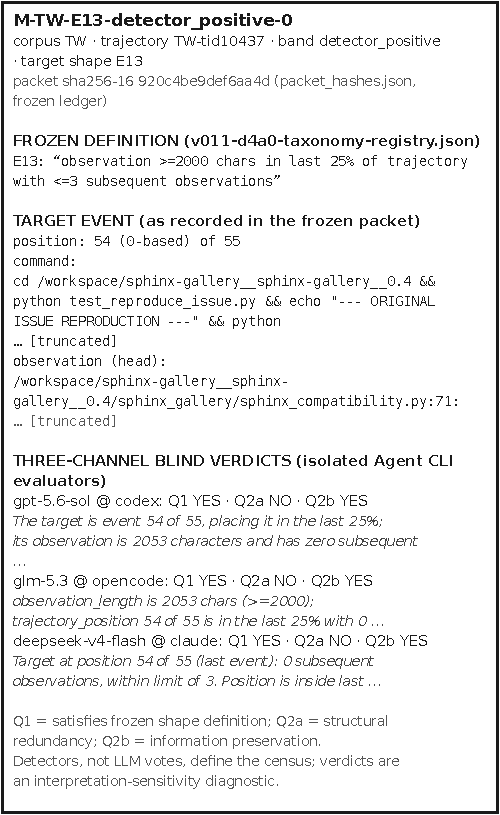
\includegraphics[width=\linewidth]{figures/fig_case_annotation_unit.pdf}
\caption{One frozen annotation unit from the 120-item $\times$ 3-evaluator formal annotation (full provenance in Supplement~B). Top: the frozen E13 definition. Middle: the target event (trajectory position 54 of 55; observation truncated for space). Bottom: the three isolated channel verdicts --- all three channels answer YES/NO/YES on Q1/Q2a/Q2b. Detectors, not LLM votes, define the census; the audit diagnoses interpretation sensitivity only.}
\label{fig:case-annotation}
\Description{A case card showing a frozen annotation packet: the E13 definition text, the target tool command and truncated observation, and three verdict rows (GPT-5.6-sol via Codex, GLM-5.3 via OpenCode, DeepSeek-V4-flash via Claude Code), each answering yes, no, yes for taxonomy membership, structural redundancy, and information preservation.}
\end{figure}

\section{Datasets and Experimental Design}

\begin{table}[t]
\centering
\caption{Evaluation matrix; the Open-SWE v1.0 strata are drawn from the Open-SWE-Traces corpus~\cite{openswetraces2026}.}
\label{tab:eval}
\footnotesize
\setlength{\tabcolsep}{3pt}
\begin{tabular}{@{}llllr@{}}
\toprule
\textbf{Corpus} & \textbf{Scaffold} & \textbf{Model} & \textbf{Sessions} & \textbf{Role} \\
\midrule
Thoughtworks & heterogeneous & source & 15{,}000 & discovery \\
Open-SWE v1.0 & OpenHands & Minimax-M2.5 & 10{,}000 & external; scaffold \\
Open-SWE v1.0 & SWE-agent & Minimax-M2.5 & 10{,}000 & external; scaffold \\
Open-SWE v1.0 & OpenHands & Qwen3.5-122B & 15{,}000 & model contrast \\
Open-SWE v1.0 & SWE-agent & Qwen3.5-122B & 20{,}334 & factorial \\
\bottomrule
\end{tabular}
\end{table}

\begin{figure}[t]
\centering
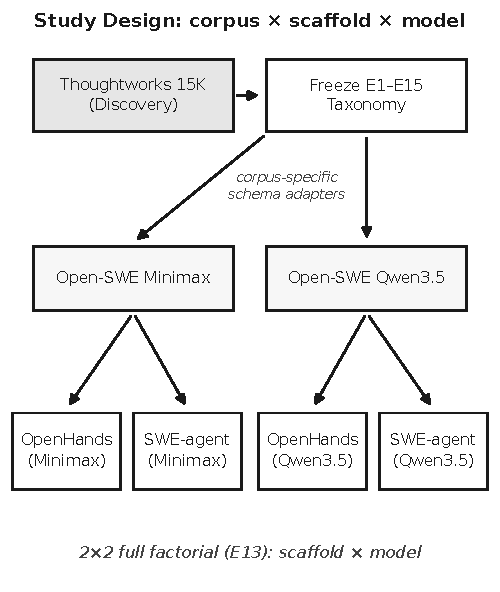
\includegraphics[width=\linewidth]{figures/fig2_design.pdf}
\caption{Study design. The frozen taxonomy is applied to all evaluation strata through corpus-specific schema adapters; the normalization-caliber effect is bounded by a same-caliber recalculation. The 2$\times$2 factorial closes the design for E13.}
\Description{Flow diagram of the study design. Two public corpora feed a frozen 15-shape taxonomy with mechanical detectors, which produces a per-shape census; a separate two-by-two factorial over scaffold and model closes the design for E13; results feed a capability mapping with SOC and COC dual-ledger coverage.}
\label{fig:design}
\end{figure}

Table~\ref{tab:eval} shows the evaluation matrix. The OpenHands\,$\times$\,Qwen3.5 stratum uses 6 of 17 available shards (15{,}000 of $\sim$35{,}000 trajectories) due to download-bandwidth constraints at data-acquisition time; the shard selection (first 6 by ordinal) was made before any analysis and is independent of trajectory content. All other strata use their full available shard set.

\textbf{Recording-time strata, not executed configurations.} All censuses in this study are offline, deterministic analyses of recorded trajectories obtained from the two public corpora. The scaffold and model columns of Table~\ref{tab:eval} are recording-time strata labels shipped with the datasets: the Open-SWE v1.0 strata were recorded by the dataset authors running OpenHands and SWE-agent with Minimax-M2.5 and Qwen3.5-122B, and the Thoughtworks sessions are recorded production trajectories from heterogeneous in-house tooling. Our measurement pipeline invokes no agent and no model at any point; the only live invocations reported in this paper are the LLM annotation audit (Supplement~B) and the online A/B evaluation (Supplement~D), each documented with its own protocol and provenance.

\textbf{Frames, not independent tasks.} Each corpus row is an \emph{observation session} produced by a model/scaffold pair over a repository snapshot. Multiple sessions can derive from the same underlying task family under different model/scaffold conditions; we therefore treat sessions as observations within a sampling frame and never as independent coding tasks. Model and scaffold contrasts are computed \emph{within} strata to avoid pseudo-replication.

\textbf{Recorded trajectories and session identifiers.} The discovery corpus ships 15{,}000 recorded trajectories under 13{,}053 unique session identifiers: 1{,}947 identifiers each appear on exactly two recorded trajectories (1,946 pairs with distinct content and one pair with identical content). All discovery-side session-level counts in this paper use recorded-trajectory (row) identity---each recorded trajectory is one observation---and identifier collisions are treated as a labeling property of the source, not as evidence about run independence. Under identifier-set counting every replication band is unchanged, with trajectory-level ratios uniformly closer to 1.0.

\textbf{Metrics.} Incidence is the fraction of recorded trajectories containing a shape (the discovery corpus has 15,000 recorded trajectories under 13,053 unique session identifiers; \S4). COC is supported registry-qualified opportunity mass divided by total registry-qualified opportunity mass, using allocation-based byte accounting with overlap control. For each session, the frozen implementation allocates observation-character mass equally across its detected shapes; denominator allocations exclude E7/E12 and other registry-ineligible shapes, and numerator allocations retain full-fit supported shapes. This is a coverage accounting proxy, not an exact byte-offset union or directly measured safely deletable bytes. SOC uses supported-session count divided by the census per-session frame, as implemented; its denominator is not recomputed. Shipped-only and shipped-plus-candidate ledgers remain separate. Capability Gap Rate uses the frozen production-to-candidate COC ratio; no ratio is recalculated. Coverage percentages are displayed to two decimal places from the stored canonical census proportions.

\section{RQ1--RQ2: Prevalence and Cross-Corpus Replication}

\begin{figure}[t]
\centering
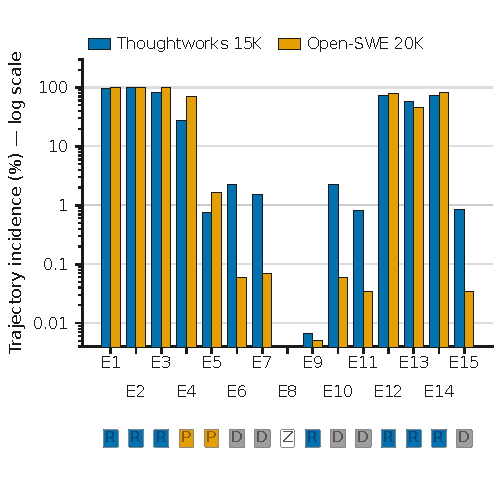
\includegraphics[width=\linewidth]{figures/fig3_incidence.pdf}
\caption{Opportunity incidence across the two corpora (discovery side: recovered full three-source parse, A1R2, counted at trajectory identity, A1R3). All six core shapes (E1, E2, E3, E12, E13, E14) satisfy the descriptive replication criterion across corpora (full-precision ratios 0.79--1.28); the five sparse shapes (E6, E7, E10, E11, E15) are DATASET\_SPECIFIC. E4 is NOT\_MEASURABLE on Open-SWE due to schema limitations. Log scale; the status row reports the frozen per-shape replication status: R (replicated), P (partial), D (dataset-specific), Z (zero baseline --- E8 is NOT\_ESTIMABLE in both corpora).}
\Description{Grouped bar chart on a logarithmic y-axis showing per-shape session incidence for shapes E1 through E15 in two corpora, Thoughtworks 15K and Open-SWE 20K. Dominant shapes E1, E2, E3, E12, E13, and E14 show high incidence in both corpora; sparse shapes show low incidence with corpus-composition-sensitive band assignments; E4 and E8 are marked not measurable in one corpus each.}
\label{fig:incidence}
\end{figure}

\subsection{RQ1: Prevalence}

\paragraph{Opportunity magnitude.} In the frozen Thoughtworks repetition-class ledger, the byte-deduplicated union of E2/E3/E14 has a median estimated removable payload of 9{,}782 chars among sessions with a qualifying union event. Across all discovery sessions, 46.7\% reach at least 5K estimated removable chars; among union-hit sessions, 93.68\% have at least eight qualifying events. These are conservative mechanical-oracle character estimates, not token savings or online benefit. They show that detector-defined repetition opportunities can be substantial and recur within a session, rather than merely appearing once.

\paragraph{E13 structural decomposition.} Under the recovered full three-source parse (A1R2) and trajectory-identity counting (A1R3), discovery-side E13 trajectory-level incidence is 58.72\%. The pre-amendment frozen decomposition records a median output of 5{,}780 chars, but only 3.5\% median mechanical-dedup removable ratio. Of E13 events in that frozen ledger, 48.55\% are final observations, while 51.45\% still have a subsequent tool call; same-artifact rereading occurs at 6.94\%. Main payload forms are diff-like, unstructured, table/list-like, and test-case lists. Late placement therefore neither establishes redundancy nor rules out future use. We treat E13 as a \emph{high-frequency semantic-folding candidate, not a mechanical-deduplication opportunity}; any semantic folding would require separate fidelity and task-benefit evidence.

Opportunities are common. The dominant large-payload shapes occur in a majority of sessions: \textbf{large diagnostics in 72.9\% (TW) / 79.5\% (OSW)} of sessions with a median observation of 8.0K chars, and \textbf{late-trajectory large outputs in 58.7\% / 46.6\%} with median 5.8K chars (p75 10.3K; TW medians from the pre-amendment frozen ledger). Repetition shapes occur in a majority of sessions: same-file rereads in \textbf{82.0\% (TW) / $\sim$100\% (OSW)} of sessions, similar-command repeats in 98.6\%/$\sim$100\%, with per-session repeat counts reaching a median of 7--24 qualifying events in the frozen repeat-family ledger. Even the low-value tail is populated---unchanged validation (0.81\%) and large build outputs (0.01\%) occur, just too rarely or too small to justify dedicated handling.

\begin{findingbox}
\textbf{Finding 1.} Natural context-compression opportunities are common in real coding-agent trajectories. Several repetition and large-output shapes occur in a substantial fraction of sessions rather than as isolated corner cases.
\end{findingbox}

\subsection{RQ2: Cross-Corpus Reproducibility}

\textbf{Answer: yes for the dominant structures.} 8 of 13 measurable shapes land in the REPLICATED (incidence ratio 0.5--2.0) or PARTIAL (0.2--0.5, 2--5) band---a pre-specified descriptive replication criterion, the 0.5--2.0 band is not a statistical equivalence interval. All six core shapes replicate, with ratios tightening toward 1.0 relative to the pre-amendment frame (E12 72.9\%\,$\rightarrow$\,79.5\%; E13 58.7\%\,$\rightarrow$\,46.6\%; E1/E2/E3/E14 full-precision ratios 1.03/1.01/1.22/1.28). The five remaining measurable shapes (E6, E7, E10, E11, E15---sparse validation-negative discoveries) are DATASET\_SPECIFIC: the klear recovery amendment (A1R2) recovered the full three-source discovery parse (+105M observation chars over 15{,}000 recorded trajectories), multiplying discovery-side validation events for these sparse shapes (e.g., E10 17\,$\rightarrow$\,297 sessions) while the external corpus stayed sparse---a corpus-composition difference, not a detector failure.

Boundary evidence is preserved: \textbf{E4 (overlapping file read) is NOT\_MEASURABLE on Open-SWE}---the corpus's tool calls do not carry read-range fields, so the detector cannot be applied. This is a schema limitation, \textbf{not} a failed replication. E6 and E9 remain rare on the Open-SWE side (15 and 1 sessions); on the recovered discovery side E6 counts 333 trajectories (2.22\%) while E9 remains a single session.

We note one detector-caliber caveat: the Open-SWE side of the E1/E2/E3/E14 comparisons uses path-aware command normalization (the tool path is appended to view/open/edit command strings before grouping), applied identically within that corpus, while the discovery side originally used the pre-registered normalization without path suffixes. A same-caliber recalculation on the pre-amendment discovery frame shifted incidence by +0.14/+0.08/+0.15/+3.74\,pp for E1/E2/E3/E14 and left every replication band unchanged (ratios 1.45--1.52); those shifts are historical pre-amendment results. The discovery census reported here reflects the recovered full three-source parse (A1R2) counted at trajectory identity (A1R3), under which the four repetition shapes are REPLICATED with full-precision ratios 1.03/1.01/1.22/1.28; same-caliber normalization re-validation under the recovered frame remains future work. RQ2's core claim therefore rests on the full 13-shape band distribution.

\begin{findingbox}
\textbf{Finding 2.} Eight of thirteen measurable opportunity structures---including all six dominant high-incidence core shapes---satisfy our descriptive replication criterion across the two corpora; the five sparse shapes are corpus-composition-sensitive.
\end{findingbox}

\section{RQ3--RQ4: Model Stability and Scaffold Modulation}

\begin{table}[t]
\centering
\caption{Core shapes: incidence by scaffold and model. All six shapes are MODEL\_STABLE.}
\label{tab:factorial}
\small
\begin{tabular}{@{}lcccc@{}}
\toprule
\textbf{Shape} & \textbf{OH MM} & \textbf{OH QW} & \textbf{SA MM} & \textbf{SA QW} \\
\midrule
E1 repeated exact cmd & .9993 & 1.0000 & .9999 & 1.0000 \\
E2 repeated similar cmd & .9995 & 1.0000 & 1.0000 & 1.0000 \\
E3 same-file reread & .9997 & 1.0000 & 1.0000 & .9991 \\
E12 large diagnostic & .7715 & .7417 & .8185 & .8292 \\
E13 late large output & .6487 & .4389 & .2840 & .2392 \\
E14 output$\rightarrow$reread & .9388 & .9833 & .9579 & .9705 \\
\bottomrule
\end{tabular}
\end{table}

\subsection{RQ3: Cross-Model Stability}

We verify model stability for the six core shapes within each scaffold, using the frozen Open-SWE frame (Table~\ref{tab:factorial}). All six shapes are MODEL\_STABLE: the largest cross-model shift is E13 within OpenHands (0.6487\,$\rightarrow$\,0.4389, ratio 0.68), still within the stability band; every other ratio lies between 0.84 and 1.013. Sparse shapes (E5--E7, E10, E11) show MODEL\_SENSITIVE verdicts, but these rest on few events and are excluded from the core narrative.

\begin{findingbox}
\textbf{Finding 3.} The dominant opportunity structures remain stable across Minimax and Qwen3.5 under both evaluated agent scaffolds.
\end{findingbox}

\subsection{RQ4: Scaffold Modulation}

E13 (late-trajectory large output) is the one core shape whose incidence moves strongly---and the movement tracks \emph{scaffold}, not model.
\begin{figure}[t]
\centering
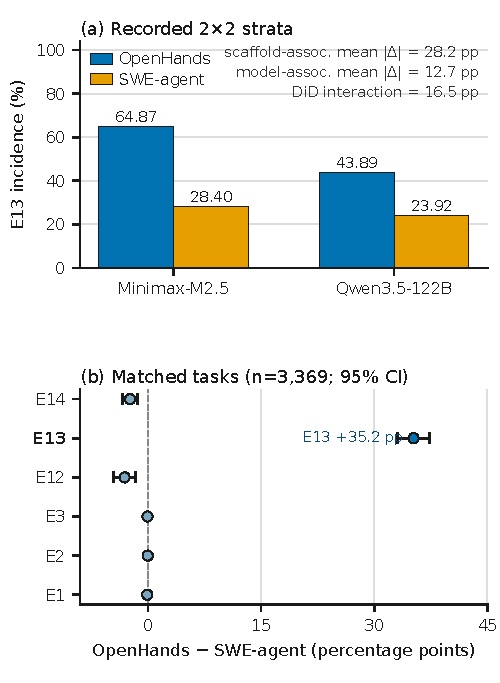
\includegraphics[width=\linewidth]{figures/fig4_e13_interaction.pdf}
\caption{E13 incidence by scaffold and model. Scaffold-associated variation (mean 28.2\,pp) exceeds model-associated variation (mean 12.7\,pp); DiD interaction 16.5\,pp. Direction-consistent across models.}
\Description{Grouped bar chart of E13 session incidence for OpenHands and SWE-agent under two models, Minimax and Qwen. OpenHands shows higher incidence than SWE-agent in both models, at roughly 64.9 versus 28.4 percent for Minimax and 43.9 versus 23.9 percent for Qwen. Annotations report mean scaffold-associated variation of 28.2 percentage points, mean model-associated variation of 12.7 percentage points, and a 16.5 percentage point DiD interaction.}
\label{fig:e13}
\end{figure}

Contrasts: scaffold-within-Minimax $-36.5$\,pp; scaffold-within-Qwen $-20.0$\,pp; model-within-OpenHands $-21.0$\,pp; model-within-SWE-agent $-4.5$\,pp. Mean scaffold-associated variation \textbf{28.2\,pp} vs.\ mean model-associated variation \textbf{12.7\,pp}; difference-in-differences interaction \textbf{16.5\,pp}---models modulate the within-frame scaffold-associated difference's magnitude without changing its direction (SA is lower within both models).

\emph{Mechanism interpretation (not a proven cause):} OpenHands' editor-centric interaction (\texttt{str\_replace\_editor view} over large files) yields more late-trajectory large observations than SWE-agent's command-oriented flow, whose observations are shorter and more fragmented.

\begin{findingbox}
\textbf{Finding 4.} Opportunity incidence can be strongly scaffold-dependent. For E13, scaffold-associated variation is larger than model-associated variation in the controlled 2$\times$2 evaluation, with consistent direction across both models.
\end{findingbox}

We phrase this as within-frame association; we do not generalize causally to all agent architectures. Interface design is a known influence on agent behavior (SWE-agent's ACI design precedent), so we report scaffold-associated modulation rather than claiming scaffold discovery.

\section{RQ5: How Much Opportunity Is Covered Today?}

\begin{figure}[t]
\centering
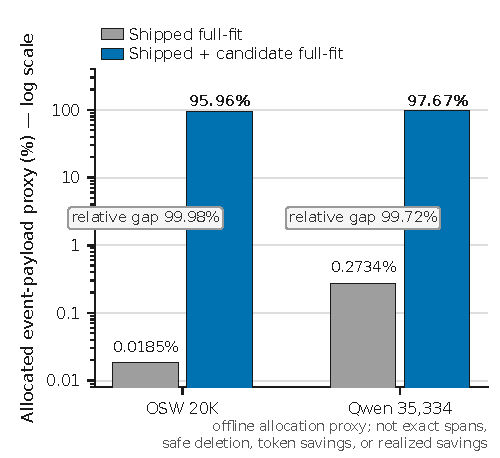
\includegraphics[width=\linewidth]{figures/fig5_coverage.pdf}
\caption{Dual-ledger capability coverage. Production (shipped-only) mechanisms cover 0.018\% of qualified allocated event-payload mass. The research candidate (RDS, default OFF) reaches 100\% session coverage and 95.96\% event-payload COC. The 99.98\% relative gap between them represents the opportunity-to-capability gap.}
\Description{Grouped bar chart of dual-ledger coverage. Session opportunity coverage is 2.07 percent for production shipped-only mechanisms and 100 percent for the research shipped-plus-candidate candidate; byte coverage with allocation-based accounting and overlap control is 0.018 percent for production and 95.96 percent for research. An annotation reports a 99.98 percent capability gap rate in bytes.}
\label{fig:coverage}
\end{figure}

Mapping shapes to capabilities: shipped mechanisms address E8-class lint outputs (structured folding), sparse validation/search shapes, and partially cover read-class shapes; the repeated-delivery band (E1/E2/E3/E14) is covered only by the RDS candidate; E12-class diagnostics are partially covered by a capability whose task-level benefit previously tested negative; E13-class semantic folding is unimplemented.

\textbf{Dual ledger (Minimax 20K):} production (shipped-only) \textbf{event-payload COC 0.018\%}; research (+RDS candidate) \textbf{event-payload COC 95.96\%}; \textbf{Relative gap 99.98\%}. The Qwen-side census yields the same structure (shipped SOC 6.12\% / COC 1.14\% vs.\ +candidate 100\% / 91.27\%)---the gap is cross-model stable.

The research ledger does \textbf{not} describe the shipped product: the RDS candidate is \texttt{CAPABILITY\_CANDIDATE / DEFAULT\_OFF}, and its online task-level benefit is not established (F1).

\begin{findingbox}
\textbf{Finding 5.} In the evaluated TASCO configuration, shipped mechanisms cover 0.018\% of qualified allocated event-payload mass, while a reversible research candidate reaches 95.96\% of qualified allocated event-payload mass---revealing a substantial opportunity-to-capability gap. The gap is not that opportunities are absent---a reversible candidate covers $\sim$90\% of qualified bytes---but that production capability has not been built for the dominant shapes.
\end{findingbox}

\section{Secondary Finding: Offline-to-Online Gap}
\label{sec:f1}

Offline replay shows abundant removable content: the RDS prototype removed \textbf{218M chars} across the 15K-trajectory discovery corpus, with \textbf{90.1\%} byte-coverage of qualified opportunity and a fully reversible representation (289{,}822 replay events, zero reconstruction failures, exact-match 1.0, oracle capture 0.8098). Figure~\ref{fig:rds-capture} decomposes the capture side of this frozen ledger.

\begin{figure}[t]
\centering
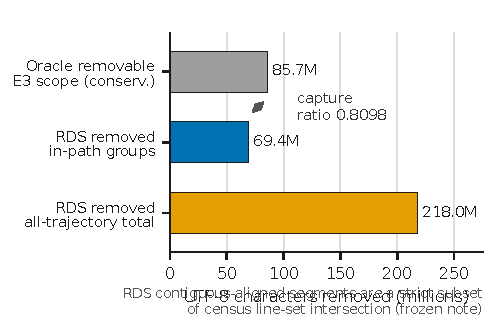
\includegraphics[width=\linewidth]{figures/fig_rds_replay_capture.pdf}
\caption{Offline replay capture (frozen byte quantities). The oracle-conservative removable E3 scope (85.7M UTF-8 chars) and the RDS in-path-groups removal (69.4M) give the oracle-capture ratio 0.8098; the all-trajectory removal total (218.0M chars) spans all shapes and is a different scope than the E3-qualified one, not a nested comparison. RDS contiguous-aligned segments are a strict subset of the census line-set intersection.}
\label{fig:rds-capture}
\Description{Horizontal bar chart of three frozen replay quantities in millions of UTF-8 characters: oracle conservative removable E3 scope 85.7M, RDS removed in-path groups 69.4M with capture ratio 0.8098 between the first two, and RDS removed all-trajectory total 218.0M.}
\end{figure}

Online, however, the same mechanism's task-level effect could not be established in a 24-pair real-agent A/B: the A/B was correctness-clean (24/24 pairs B-pass/T-pass, zero attributable failures, no recovery backlash), yet the aggregate +7.38\% was statistically indistinguishable from label randomization (permutation $p = 0.1185$), with only 54\% non-negative pairs.

The mechanism audit traces this to signal-to-noise, not to the primitive: \textbf{within-task replicate pairs swing by a median 27.96\%} of session tokens---exceeding the median paired B/T delta (23.79\%)---while the mechanism's token exposure is a median \textbf{0.011\%} of session tokens (signal:noise 0.0003). Under this noise, no replication count $\leq$10/arm reaches 0.80 simulation-based detection probability under our decision criterion for +3\%/+5\% effects. An independent 60K-trajectory stochasticity study~\cite{randomness2026} corroborates this finding, recommending multi-run evaluation with power analysis for sparse-activation mechanisms.

The simulation counts a trial as detected when its estimate has the target direction and an absolute magnitude at least half the injected effect. The frozen resampling pools within-arm noise; it is not a significance-test rejection probability. Supplement D preserves the exact procedure. Table~\ref{tab:qualification} condenses the three qualification attempts; the detailed frozen ledger is in Supplement~D.

\begin{table}[t]
\centering
\caption{Online qualification attempts behind the offline-to-online gap reading (frozen ledger; details in Supplement~D).}
\label{tab:qualification}
\small
\begin{tabular}{@{}p{0.21\linewidth}p{0.44\linewidth}p{0.25\linewidth}@{}}
\toprule
\textbf{Attempt} & \textbf{Key frozen quantities} & \textbf{Verdict} \\
\midrule
D3-E7 simulation design & within-task noise median 27.96\%; signal:noise 0.0003; power 0.622/0.699/0.856 at $+3/+5/+10$\% effects & underpowered for $+3/+5$\% effects at $\leq$10/arm \\
D3-E5 RDS A/B & 24 pairs; oracle 24/24; aggregate $+7.38$\%; 13/24 non-negative; permutation $p = 0.1185$ & G2 FAIL \\
V0.11-D2 terminal-state & 18 pairs; opportunity incidence 0.0; aggregate $-0.0805$ & NOT\_QUALIFIED \\
\bottomrule
\end{tabular}
\end{table}

The distinction matters: opportunity exists (RQ1), the mechanism can compress reversibly (offline replay), the mechanism was delivered online without harm (A/B), and no task-level effect was observed---but the \emph{task-level effect} is buried under trajectory variance at practical sample sizes.

\begin{findingbox}
\textbf{Finding 6.} Offline compressibility should not be interpreted as online task-level savings without accounting for mechanism exposure and trajectory variance.
\end{findingbox}

\section{Discussion}

\textbf{Opportunity-aware compression.} The taxonomy implies compression policy should select primitives by trajectory shape---reference-based suppression for repeated deliveries, terminal folding for end-of-task summaries, preservation-aware handling for decision-critical diagnostics---rather than apply a uniform token threshold.

\textbf{Scaffold belongs in the benchmark.} Because incidence can be scaffold-modulated (2.3$\times$ for E13 at fixed model), compression evaluations should report the agent scaffold alongside the backbone model; a capability qualified on one scaffold cannot be assumed to transfer.

\textbf{The semantic frontier.} The largest uncovered shape (E13, $\sim$50\% incidence) is mechanically redundant by only 3.5\%; its value lies in semantic structure---diffs, test-result lists, structured diagnostics---which requires folding with information-preservation gates. That is a distinct primitive, deliberately out of scope here.

\textbf{From measurement to system design.} These findings are the design inputs for a runtime that dispatches shape-appropriate primitives at delivery points, registers anchors for reversibility, and reports per-shape exposure against trajectory noise---the design brief for our companion system work.

\section{Threats to Validity / Limitations}

\textbf{Construct validity.} The taxonomy is mechanically reproducible, but natural-language interpretation across shapes is uneven: overall Q1 agreement is 52.65\% ($\kappa=0.2665$) and Q2 agreement is 49.41\% ($\kappa=0.2284$), compared with E13 Q1/Q2 agreement of 96.4\%/78.6\% ($\kappa=0.9146$ for E13 Q1). The reconciled heterogeneous-model audit is an interpretation-sensitivity diagnostic, not human ground truth or evidence of detector precision or safe compression.

\textbf{Schema limitation.} E4 is NOT\_MEASURABLE on Open-SWE (no read-range fields); this is a schema gap, not evidence that overlapping reads do not occur.

\textbf{Internal validity.} The 2$\times$2 controls scaffold and model, but unmeasured within-scaffold confounders may remain; the 16.5\,pp interaction shows model-dependent effect magnitude. Scaffold and model contrasts are measured over recording-time strata rather than fresh executions; recording-time confounders (harness versions, decoding parameters, dataset curation) may contribute to the observed scaffold association.

\textbf{External validity.} Both corpora are coding-agent SWE/PR workloads across nine languages; other task families and non-coding domains are untested.

\textbf{Low-incidence noise.} MODEL\_SENSITIVE verdicts on sparse shapes (E5--E7, E10, E11) rest on few events and should not be over-interpreted. Sparse-shape replication bands are also corpus-composition-sensitive: the klear recovery amendment (A1R2) multiplied discovery-side validation events for E6/E7/E10/E11/E15 while the external corpus stayed sparse, flipping their bands to DATASET\_SPECIFIC. Band assignments for shapes with fewer than 300 discovery-side sessions should be read as order-of-magnitude statements.

\textbf{Coverage boundary.} The fifteen shapes do not exhaust observation content: large unmatched outputs are accounted as residuals The OpenCode+GLM-5.3 channel had a 51.7\\% cell-level output gap concentrated on E14 items, reflecting GLM-5.3 reasoning-model latency on paired-context packets. The OpenCode+GLM-5.3 channel had a 51.7\% cell-level output gap concentrated on E14 (output$\rightarrow$reread) items, reflecting GLM-5.3 reasoning-model latency on paired-context packets rather than definition ambiguity. (Supplement~A), not as incompressible content. The current detectors are by construction insensitive to some single-delivery structured outputs and to cross-trajectory repetition; the residual pool motivates post-hoc hypotheses to be validated on future datasets, not a validated taxonomy extension.

\textbf{Online evaluation.} Offline compressibility does not imply online savings (F1); the candidate's task-level benefit is NOT\_ES\-TAB\-LISHED.

\textbf{Session identity.} Discovery-side session identifiers are not unique: the 15{,}000 recorded trajectories carry 13{,}053 unique identifiers (1,947 identifiers on two recorded trajectories each; \S4). All discovery-side session-level statistics therefore use trajectory-level (row) identity; under identifier-set counting every replication band is unchanged and coverage is at most 1,947 trajectories per shape lower.

\textbf{Detector caliber.} The external (Open-SWE) side applies path-aware command normalization; the discovery (TW) side originally did not. A same-caliber recalculation of E1/E2/E3/E14 on all 15{,}000 TW sessions under the path-aware rule shifts incidence by at most 3.74\,pp (E14; E1/E2/E3 $\leq$0.15\,pp) and leaves every replication band unchanged. The corpus-specific schema adapters themselves (structured tool-call fields vs.\ code-fence fallbacks, user-role observation capture on TW) remain a per-corpus property and are not exercised by this recalculation; only session incidence is recalculated, not removable-char ledgers. The discovery-side primary numbers reported in this paper reflect the klear recovery amendment (A1R2), which recovered the full three-source parse of the discovery corpus, and the trajectory-identity caliber (A1R3); same-caliber normalization re-validation under the recovered frame remains optional future work.

\section{Related Work}

\textbf{Agent context compression and trajectory reduction.} AgentDiet~\cite{agentdiet2026} manually analyzes 100 Trae-Agent trajectories, classifies waste into useless/redundant/expired categories, and reduces trajectory cost across two LLMs and two benchmarks---the closest prior work to our measurement. AttnCompress~\cite{attncompress2026} introduces attention-guided dynamic trajectory compression for SWE-bench; Paritok-4B~\cite{paritok4b2026} trains an extractive intent-conditioned compressor over 67K OpenHands trajectories; SWE-Pruner~\cite{swepruner2026} prunes task-relevant code context; TACO~\cite{taco2026} self-evolves terminal-observation compression rules; CORVUS~\cite{corvus2026} addresses file-state synchronization to prevent stale rereads; Squeez~\cite{squeez2026} learns minimal verbatim evidence retention for tool outputs; ACON~\cite{acon2026} compresses observations and interaction history; ReSum~\cite{resume2025} and AgentFold~\cite{agentfold2025} apply periodic summarization to web agents. All of these answer \emph{how to compress}; none characterizes the \emph{opportunity surface} itself: none derives a frozen opportunity taxonomy, replicates it across corpora, or maps it to capability coverage.

\textbf{Coding-agent evaluation and benchmarks.} SWE-bench~\cite{swebench2024}, SWE-agent~\cite{sweagent2024}, OpenHands~\cite{openhands2024}, Multi-SWE-Bench~\cite{multiswebench2026}, and SWE-Gym~\cite{swegym2025} evaluate task correctness on real repositories. SWE-agent's ACI design established that interface choices shape agent behavior---a precedent we cite for RQ4 rather than claim as novel. We use these systems and datasets as \emph{trajectory} corpora: task benchmarks evaluate correctness, while trajectory corpora expose compression opportunity.

\textbf{Empirical analysis of agent trajectories.} Process-Centric Analysis~\cite{processcentric2025} characterizes 4{,}000 trajectories across two scaffolds and four backbones using Graphectory process metrics; Failure-as-a-Process~\cite{failureprocess2026} anatomizes 3{,}843 CLI-agent trajectories across seven models and three scaffolds into 14 failure findings; a harness-design study~\cite{harnessdesign2026} ablates 176 matched settings across four models; Understanding SE Agents~\cite{understandingseagents2025} extracts behavioral motifs from 120 trajectories; a 60K-trajectory stochasticity study~\cite{randomness2026} independently recommends multi-run evaluation with power analysis---corroborating our F1. Agent Trajectories as Programs~\cite{trajectoriesprograms2026} fingerprints procedure differences across ten agents. These studies characterize agent behavior, process quality, failures, and difficulty---but none derives a fine-grained compression-opportunity taxonomy with frozen detectors, replicates it across independent corpora, or maps it to capability coverage.

\textbf{Position.} Prior work has identified broad forms of waste in coding-agent trajectories and proposed mechanisms to reduce them. What is still missing---and what this paper provides---is a systematic and reproducible measurement of naturally occurring context-compression opportunities, moving beyond prior qualitative waste analyses and compression-mechanism evaluations through a fine-grained detector-backed taxonomy, cross-corpus replication, controlled model\,$\times$\,scaffold validation, and opportunity-to-capability coverage analysis.

\section{Conclusion}

Coding-agent trajectories contain abundant naturally occurring context-compression opportunities. The core opportunity structures satisfy our descriptive replication criterion across two independent public corpora---with full-precision incidence ratios 0.79--1.28---and remain largely stable across backbone models within both evaluated scaffolds, while their incidence can be substantially modulated by agent scaffold design. Existing deployed mechanisms cover only a small fraction of this opportunity space---a 99.98\% relative allocation gap under our dual-ledger measurement---indicating that future compression systems should be designed around empirically observed workload structure and scaffold behavior rather than generic token reduction. The frozen taxonomy, detectors, manifests, and coverage ledgers are released in our artifact repository\footnote{\url{https://github.com/sunSUNQ/compression-opportunities} (see Artifact Availability).} to make the next compression primitive measurable before it is built.

\section*{Artifact Availability}

All frozen artifacts supporting this paper are publicly available at \url{https://github.com/sunSUNQ/compression-opportunities}: the paper PDF and \LaTeX{} source; the frozen E1--E15 taxonomy and capability-mapping registry; the verbatim census, replay, and audit tools; all pre-registrations; the complete evidence pack (census results, sample manifests with SHA-256 pins, reconciliation packages, the claim trace, and the RQ--evidence matrix); both annotation-audit datasets (the 340-item two-arm audit and the 120-item $\times$ 3-evaluator formal annotation); all figures and figure data; and Supplements~A--D. The two upstream corpora are public on Hugging Face (\url{https://huggingface.co/datasets/thoughtworks/agentic-coding-trajectories} and \url{https://huggingface.co/datasets/nvidia/Open-SWE-Traces}); each census manifest pins the exact sample it consumed, and every published number traces to a stored artifact.


\nocite{costattribution2026,iclr_compression2026,acm_acm2026,difficulty2026,contextrot2026,hasmem2026,trace2026,summariesdistort2026}
%
% BibTeX wired 2026-10-09 (PAPER-LAYOUT-PREFLIGHT): ACM-Reference-Format,
% citation-order numbering; the 8 \nocite entries are inventory works without
% inline anchors; md-list entry [4] (arXiv:2608.16370) is NOT in refs.bib
% (no author metadata in frozen evidence) and is therefore not rendered.
\section*{Acknowledgments}
The author thanks the maintainers of the open-source agent frameworks and public corpora that made this measurement possible. The LLM systems named in this paper were used as annotation agents under a fixed, blinded protocol; they are the object of study, not co-authors. All methodology, analysis, and conclusions are the author's own.

\bibliographystyle{ACM-Reference-Format}
\def\bibfont{\footnotesize}
\setlength{\bibsep}{2.5pt}
\bibliography{refs}
\vfill

\end{document}
